\documentclass[12pt]{article}
\usepackage{amsmath, amssymb, enumitem, fancyhdr, graphicx, libertine, nth,
pgfplots, tikz, units, xcolor}
\pgfplotsset{compat=1.11}
\usepackage[margin=1in]{geometry}
\usepackage[libertine]{newtxmath}
\definecolor{solution-color}{HTML}{000080}
\pagestyle{fancy}
\chead{\emph{EC201 -- Problem Set 2 Solutions}}

% Define new topic command
\newcommand{\topic}[1]{\medskip\begin{center}\large\textsc{#1}\normalsize
  \end{center}}

% Define question counter:
\newcounter{question}[section]
\newcommand{\question}[1]{\refstepcounter{question}
  \subsubsection*{Question~\thequestion~-- #1}}

% Subquestions are enumerate with letters
\newenvironment{subquestions}{
  \begin{enumerate}[label=(\roman*)]}{\end{enumerate}}

\begin{document}
\topic{Choice and Demand}
\question{Neutral Goods}
Revisiting the preferences from Question 6 on the previous problem set, suppose
that you enjoy good 1 but you are neutral about good 2 (your indifference
curves are vertical lines).
\begin{subquestions}
  \item Find the demand functions $x_1\left( p_1,p_2,m \right)$ and $x_2\left(
    p_1,p_2,m \right)$.
    \par
    \textcolor{solution-color}{
      With these preferences you will spend all your money on good 1 and none
      on good 2. Therefore you demand functions would be:
      \begin{align*}
        x_1\left( p_1,p_2,m \right) &= \frac{m}{p_1}\\
        x_2\left( p_1,p_2,m \right) &= 0
      \end{align*}
    }
  \item Write down a utility function $u\left( x_1,x_2 \right)$ that would be
    consistent with these preferences.
    \par\textcolor{solution-color}{
      A utility function that would be consistent with these preferences is:
      \[
        u\left( x_1,x_2 \right)= x_1
      \]
      There are many functions that would work here, as long as they satisfied
      the following properties:
      \begin{itemize}
        \item Utility increased as $x_1$ increased.
        \item Utility does not change as $x_2$ changes.
      \end{itemize}
    }
\end{subquestions}

\question{Cobb-Douglas Demand}
Suppose you have the following utility function for goods 1 and 2:
\[
  u\left( x_1,x_2 \right) = 2 x_1^{\frac{1}{4}}x_2^{\frac{3}{4}}
\]
\begin{subquestions}
  \item Find the demand functions $x_1\left( p_1,p_2,m \right)$ and $x_2\left(
    p_1,p_2,m \right)$.

    \textcolor{solution-color}{
      At the optimum, $\left| MRS \right|=\frac{p_1}{p_2}$:
      \begin{align*}
        \frac{MU_1}{MU_2} &= \frac{p_1}{p_2} \\
        \frac{\frac{\partial u\left(x_1,x_2 \right)}{\partial x_1}}
             {\frac{\partial u\left(x_1,x_2 \right)}{\partial x_1}} &=
             \frac{p_1}{p_2} \\
             \frac{\frac{2}{4}x_1^{\frac{1}{4}-1}x_2^{\frac{3}{4}}}
             {\frac{6}{4}x_1^{\frac{1}{4}}x_2^{\frac{3}{4}-1}}
             &= \frac{p_1}{p_2} \\
             \frac{2 x_1^{-1}}
             {6x_2^{-1}}
             &= \frac{p_1}{p_2} \\
             \frac{1}{3}\frac{x_2}{x_1} &=\frac{p_1}{p_2}
      \end{align*}
      So $x_2 = \frac{3p_1x_1}{p_2}$. Inserting this into the budget
      constraint:
      \begin{align*}
        p_1x_1 + p_2x_2 &= m \\
        p_1x_1 + p_2 \left( \frac{3p_1x_1}{p_2} \right) &= m \\
        p_1x_1 + 3x_1p_1 &= m \\
        4x_1p_1 &= m \\
        x_1 &= \frac{m}{4p_1}
      \end{align*}
      Then $x_2 = \frac{3p_1}{p_2}x_1 = \frac{3p_1}{p_2}\left(
      \frac{m}{4p_1} \right)= \frac{3}{4}\frac{m}{p_2}$.
      Therefore the demand functions are:
      \begin{align*}
        x_1\left( p_1,p_2,m \right) &= \frac{m}{4p_1} \\
        x_2\left( p_1,p_2,m \right) &= \frac{3m}{4p_2}
      \end{align*}
    }
  \item The price of good 1 is \$1 and the price of good two is \$3. You have
    \$60 to spend. How much will you consume of goods 1 and 2?

    \textcolor{solution-color}{
      Using these numbers in the demand functions:
      \begin{align*}
        x_1&= \frac{m}{4p_1} = \frac{60}{4\times 1}=15\\
        x_2&= \frac{3m}{4p_2} = \frac{3\times 60}{4\times 3} = 15
      \end{align*}
    }
  \item How much of goods 1 and 2 will you buy if you had \$120 and the prices
    stayed the same? Are the goods normal or inferior?

    \textcolor{solution-color}{
      Using these numbers in the demand functions:
      \begin{align*}
        x_1&= \frac{m}{4p_1} = \frac{120}{4\times 1}=30\\
        x_2&= \frac{3m}{4p_2} = \frac{3\times 120}{4\times 3} = 30
      \end{align*}
    }
  \item If the price of good 2 doubled (to \$6), what would happen to your
    demand for good 1?

    \textcolor{solution-color}{
      Since $p_2$ doesn't enter into the demand function for good 1, nothing
      will happen to the demand for good 1.
    }
  \item Which of the following statements is true and why?
    \begin{itemize}
      \item Good 1 is a substitute to good 2.
      \item Good 1 is a complement to good 2.
      \item Good 1 is neither a substitute nor a complement to good 2.
    \end{itemize}

    \textcolor{solution-color}{
      Since the demand for good 1 doens't change in response changes in the
      price of good 2, good 1 is neither a substitute nor a complement to good
      2.
    }
\end{subquestions}

\question{Income and Substitution Effects}
Suppose your utility function is $u\left( x_1,x_2 \right)=x_1^{\frac{2}{3}}x_2^{\frac{1}{3}}$. It can be shown that the resulting demand functions are $x_1\left( p_1,p_2,m \right)=\frac{2m}{3p_1}$ and $x_2\left( p_1,p_2,m \right)=\frac{m}{3p_2}$ (you should check this). Throughout this question, you have income of $m=30$.
\begin{subquestions}
  \item If $p_1=1$ and $p_2=1$, how much of goods 1 and 2 would you buy? Sketch the budget line and optimal bundle on a graph.
  \par\textcolor{solution-color}{
    You would buy $x_1=\frac{2\time 30}{3\times 1}=20$ of good 1 and $x_2=\frac{30}{3\times 1}=10$ of good 2. See the first graph below.
  }
  \item If the price of good 1 increases to $p_1=2$ and the price of good 2 remains at $p_2$, how much of goods 1 and 2 would you buy? Sketch the new budget line and optimal bundle on your graph.
  \par\textcolor{solution-color}{
    You would buy $x_1=\frac{2\time 30}{3\times 2}=10$ of good 1 and $x_2=\frac{30}{3\times 1}=10$ of good 2. See the second graph below.
  }
  \item Suppose that after the price of good 1 increased, the government gave you just enough money so that you could afford the original bundle, i.e.~the bundle in part(i). How much money would the government need to give you?
  \par\textcolor{solution-color}{
    With the new prices, the slope of the budget line is -2. We know the budget line after the government handout needs to pass through the point $\left( 20,10 \right)$ as that was your original bundle. Since a government handout is like a change in income, the budget line will have the same slope of -2. We know therefore that the budget line satisfies:
    \begin{equation*}
      x_2 = a - 2 x_1
    \end{equation*}
    where $a$ is the vertical intercept. Since we know $\left( 20,10 \right)$ is a point on this line, we can use that to solve for the vertical intercept:
    \begin{equation*}
      10=a-2\times 20 \Longrightarrow a = 10+2\times 20 = 10+40 = 50
    \end{equation*}
    The new budget line is therfore:
    \begin{equation*}
      x_2 = 50 - 2x_1
    \end{equation*}
    The vertical intercept is 50 and the horizontal intercept is 25. This is shown in the third graph below. Since $p_2=1$ and the vertical intercept is $\frac{m}{p_2}$, we know your income must be 50. Since your income was initially 30, the government would need to give you 20 to allow you to afford your initial bundle.
  }
  \item If the government gave you this reimbursement, how much of goods 1 and 2 would you buy? Is this different from part (i)? Sketch your new budget line after the government handout and the optimal bundle.
    \par\textcolor{solution-color}{
      Going back to our demand functions with $m=50$, we get $x_1=\frac{2m}{3p_1}=\frac{2\times 50}{3 \times 2} = \frac{100}{6}=16\frac{2}{3}$ and $x_2=\frac{m}{3p_2} = \frac{50}{3\times 1} = 16\frac{2}{3}$. Your new bundle is at $\left( 16\frac{2}{3},16\frac{2}{3} \right)$. Before you bought $\left( 20,10 \right)$ so your bundle does change as $\left( 16\frac{2}{3},16\frac{2}{3} \right)$ gives higher utility (if you calculate the utilities you get $16\frac{2}{3}$ utility with the new bundle, and 15.87 with the old bundle).
    }
  \item What is the income effect and substitution effect of the price increase of good 1 on the demand for good 1?
    \par\textcolor{solution-color}{
      The substitution effect of the price change made your demand go from 20 to $16\frac{2}{3}$. The income effect is the remaining effect of going from $16\frac{2}{3}$ to 10. So the substitution effect is $3\frac{1}{3}$ ($\frac{1}{3}$ of the total effect) and the income effect is $6\frac{2}{3}$ ($\frac{2}{3}$ of the total effect).
    }
\end{subquestions}

\begin{center}
  \begin{tikzpicture}[scale=0.12]
    \draw [thick] (0,0) -- (51,0);
    \draw [thick] (0,0) -- (0,51);
    \node [right] at (51,0) {$x_1$};
    \node [above] at (0,51) {$x_2$};
    \draw [thick] (10,22) to [out=305,in=165] (30,5);
    \draw [thick] (0,30) -- (30,0);
    \draw[fill] (20,10) circle [radius =0.5];
    \draw[dotted,thick](20,0)--(20,10);
    \draw[dotted,thick](0,10)--(20,10);
    \node [below] at (30,0) {30};
    \node [left] at (0,30) {30};
    \node [below] at (20,0) {20};
    \node [left] at (0,10) {10};
  \end{tikzpicture}
  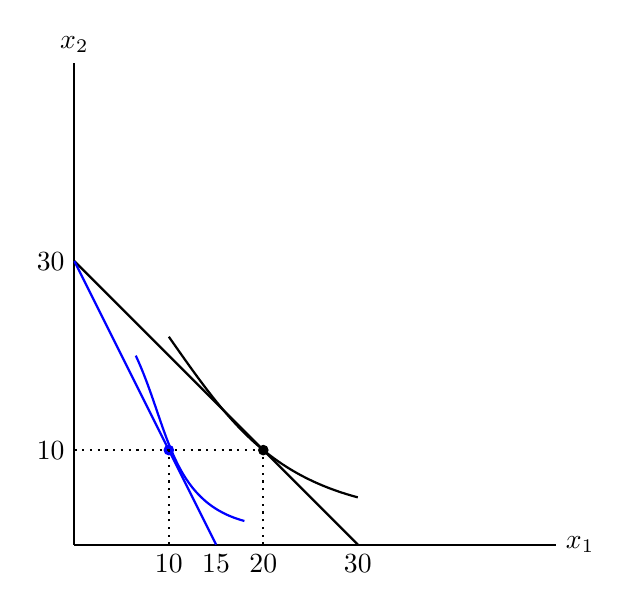
\begin{tikzpicture}[scale=0.12]
    \draw [thick] (0,0) -- (51,0);
    \draw [thick] (0,0) -- (0,51);
    \node [right] at (51,0) {$x_1$};
    \node [above] at (0,51) {$x_2$};
    \draw [thick] (10,22) to [out=305,in=165] (30,5);
    \draw [thick,blue] (6.5,20) to [out=295,in=165] (18,2.5);
    \draw [thick] (0,30) -- (30,0);
    \draw [thick,blue] (0,30) -- (15,0);
    \draw[fill] (20,10) circle [radius =0.5];
    \draw[fill,blue] (10,10) circle [radius =0.5];
    \draw[dotted,thick](20,0)--(20,10);
    \draw[dotted,thick](10,0)--(10,10);
    \draw[dotted,thick](0,10)--(20,10);
    \node [below] at (30,0) {30};
    \node [left] at (0,30) {30};
    \node [below] at (20,0) {20};
    \node [below] at (15,0) {15};
    \node [below] at (10,0) {10};
    \node [left] at (0,10) {10};
  \end{tikzpicture}
  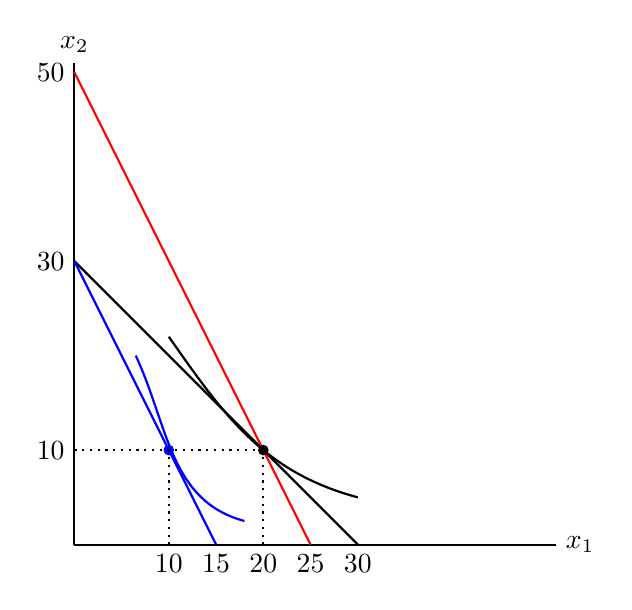
\begin{tikzpicture}[scale=0.12]
    \draw [thick] (0,0) -- (51,0);
    \draw [thick] (0,0) -- (0,51);
    \node [right] at (51,0) {$x_1$};
    \node [above] at (0,51) {$x_2$};
    \draw [thick] (10,22) to [out=305,in=165] (30,5);
    \draw [thick,blue] (6.5,20) to [out=295,in=165] (18,2.5);
    \draw [thick] (0,30) -- (30,0);
    \draw [thick,blue] (0,30) -- (15,0);
    \draw [thick,red] (0,50) -- (25,0);
    \draw[fill] (20,10) circle [radius =0.5];
    \draw[fill,blue] (10,10) circle [radius =0.5];
    \draw[dotted,thick](20,0)--(20,10);
    \draw[dotted,thick](10,0)--(10,10);
    \draw[dotted,thick](0,10)--(20,10);
    \node [left] at (0,30) {30};
    \node [left] at (0,50) {50};
    \node [left] at (0,10) {10};
    \node [below] at (30,0) {30};
    \node [below] at (20,0) {20};
    \node [below] at (10,0) {10};
    \node [below] at (15,0) {15};
    \node [below] at (25,0) {25};
  \end{tikzpicture}
  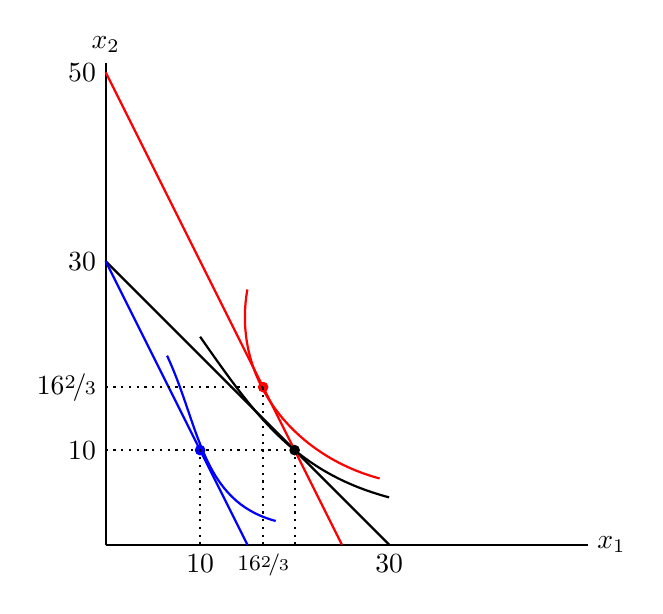
\begin{tikzpicture}[scale=0.12]
    \draw [thick] (0,0) -- (51,0);
    \draw [thick] (0,0) -- (0,51);
    \node [right] at (51,0) {$x_1$};
    \node [above] at (0,51) {$x_2$};
    \draw [thick] (10,22) to [out=305,in=165] (30,5);
    \draw [thick,blue] (6.5,20) to [out=295,in=165] (18,2.5);
    \draw [thick,red] (15,27) to [out=260,in=165] (29,7);
    \draw [thick] (0,30) -- (30,0);
    \draw [thick,blue] (0,30) -- (15,0);
    \draw [thick,red] (0,50) -- (25,0);
    \draw[fill] (20,10) circle [radius =0.5];
    \draw[fill,blue] (10,10) circle [radius =0.5];
    \draw[fill,red] (16.67,16.67) circle [radius =0.5];
    \draw[dotted,thick](20,0)--(20,10);
    \draw[dotted,thick](10,0)--(10,10);
    \draw[dotted,thick](0,10)--(20,10);
    \draw[dotted,thick](0,16.67)--(16.67,16.67);
    \draw[dotted,thick](16.67,0)--(16.67,16.67);
    \node [left] at (0,30) {30};
    \node [left] at (0,50) {50};
    \node [left] at (0,10) {10};
    \node [left] at (0,16.67) {$16\nicefrac{2}{3}$};
    \node [below] at (30,0) {30};
    % \node [below] at (20,0) {20};
    \node [below] at (10,0) {10};
    % \node [below] at (15,0) {15};
    % \node [below] at (25,0) {25};
    \node [below] at (16.67,0) {\footnotesize $16\nicefrac{2}{3}$};
  \end{tikzpicture}
\end{center}
\newpage
\topic{Intertemporal Choice}
\question{Saving for Retirement}
There are two time periods. In period 1 you work and earn income $m_1$. In
period 2 you are retired and earn no income ($m_2=0$). The interest rate is $r$
and there is no inflation. Your consumption in time periods 1 and 2 are $c_1$
and $c_2$ respectively.

The lifetime budget constraint is therefore:
\[
  c_1 + \frac{c_2}{1+r} = m_1
\]
Your lifetime utility function is:
\[
  u\left( c_1,c_2 \right)=\frac{1}{2}c_1^2 + \frac{\beta}{2}c_2^2
\]
where $\beta$ is a constant.
\begin{subquestions}
  \item Sketch the budget constraint on a graph. Label the axis intercepts and
    the endowment.
    \textcolor{solution-color}{
        \begin{tikzpicture}[baseline]
          \begin{axis}[axis equal,
                       ticks=none,
                       xmax=3,xmin=0,
                       ymin=-1,ymax=5,
                       xlabel=$c_1$,ylabel=$c_2$,
                       domain = 0:4,
                       axis x line = middle,
                       axis y line = middle,
                       width=10cm,
                       anchor=center]
            \addplot[samples=1000, restrict y to domain = 0:4] {2 - x};
            \draw (0, 2) node [left] {\scriptsize{$\left( 1+r \right)m_1$}};
            \draw (2, 0) node [below] {\scriptsize{$\;\;\;m_1$}};
            \draw (1.2, 0.9) node [right] {Slope: $-\left( 1+r \right)$};
            \draw (2, 0) node {\textbullet};
            \draw (1.9, 0.2) node [above, right] {$\left( m_1,m_2 \right)$};
          \end{axis}
        \end{tikzpicture}
    }
  \item The marginal rate of substitution of consumption between the two
    periods is:
    \[
      MRS = - \frac{\frac{\partial u\left( c_1,c_2 \right)}{\partial c_1}}
                   {\frac{\partial u\left( c_1,c_2 \right)}{\partial c_2}}
    \]
    Calculate the $MRS$ for the lifetime utility function $u\left( c_1,c_2
    \right)$ provided above.
    \textcolor{solution-color}{
      \begin{align*}
      MRS &= - \frac{\frac{\partial u\left( c_1,c_2 \right)}{\partial c_1}}
                   {\frac{\partial u\left( c_1,c_2 \right)}{\partial c_2}}\\
                   &= - \frac{c_1}{\beta c_2}
      \end{align*}
    }
  \item Now we want to find exactly how much you will want to save in the first
    period. In what follows, \underline{assume that $\beta = \frac{1}{1+r}$}
    (this will make the algebra easier).

    At the optimum you will set the $MRS$ equal to the slope of the budget
    constraint, which is $-\left( 1+r \right)$.
    Therefore we have two equations to find $c_1$ and $c_2$:
    \begin{align}
      \frac{\frac{\partial u\left( c_1,c_2 \right)}{\partial c_1}}
           {\frac{\partial u\left( c_1,c_2 \right)}{\partial c_2}} &=
           1+r  \\
             c_1 + \frac{c_2}{1+r} &= m_1
    \end{align}
    Using these two equations, solve for $c_1$ and $c_2$ as a function of $m_1$
    and $r$.

    \textcolor{solution-color}{
      The first equation is:
      \begin{align*}
      \frac{c_1}{\beta c_2} &= 1+r \\
      \frac{c_1}{c_2} &=\beta \left(1+r\right)
      \end{align*}
      Since $\beta=\frac{1}{1+r}$, we know that $\beta\left( 1+r \right)=1$.
      Then this becomes $c_1=c_2$. Putting this in the budget constraint:
      \begin{align*}
         c_1 + \frac{c_2}{1+r} &= m_1 \\
         c_1 + \frac{c_1}{1+r} &= m_1 \\
         c_1 \left( 1+\frac{1}{1+r} \right) &= m_1 \\
         c_1 \left( \frac{1+r}{1+r}+\frac{1}{1+r} \right) &= m_1 \\
         c_1 \left( \frac{2+r}{1+r}\right) &= m_1 \\
         c_1  &= m_1\left( \frac{1+r}{2+r}\right) \\
      \end{align*}
    }
  \item If the interest rate increases, will you consume more or less in the
    first period?  To answer this you can assume that $m_1=1$ and $r$ ranges
    from 0 to 1.

    \textcolor{solution-color}{
      If we plot $r$ against $\frac{1+r}{2+r}$, we get:
      \\
      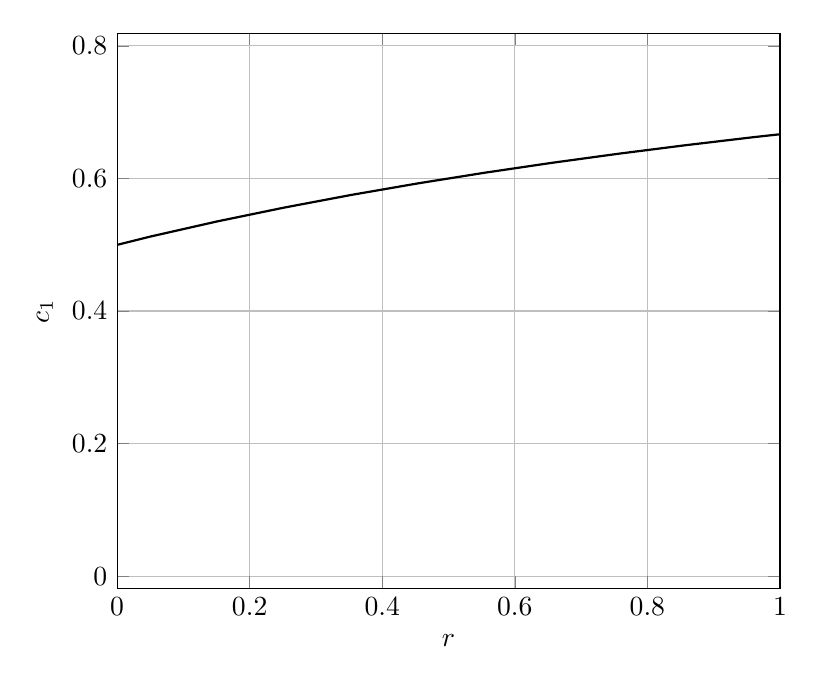
\begin{tikzpicture}[baseline]
        \begin{axis}[axis equal,
                     grid=both,
                     xmax=1,xmin=0,
                     ymin=0,ymax=0.8,
                     xlabel=$r$,ylabel=$c_1$,
                     width=10cm,
                     anchor=center]
          \addplot[thick, samples=100] {(1+x)/(2+x)};
        \end{axis}
      \end{tikzpicture}
      \\
      From this we can see that as $r$ increases, the amount of consumption in
      the first period increases.
    }
\end{subquestions}
\topic{Uncertainty}
% \question{Preferences for Risk}
% For each of the utility functions for wealth below, sketch them and state
% whether the consumer is risk averse, risk loving, or risk neutral.
% \begin{subquestions}
%   \item $u\left( W \right)=aW$, where $a>0$.
% 
%     \textcolor{solution-color}{
%       \begin{tikzpicture}[baseline]
%         \begin{axis}[axis equal,
%                      grid=both,
%                      xmax=1,xmin=0,
%                      ymin=0,ymax=0.8,
%                      xlabel=$W$,ylabel=$u\left( W \right)$,
%                      width=10cm,
%                      anchor=center]
%           \addplot[thick, samples=100] {x)};
%         \end{axis}
%       \end{tikzpicture} \\
%       This is a linear function so the consumer is risk neutral.
%     }
%   \item $u\left( W \right)=W^2$
% 
%     \textcolor{solution-color}{
%       \begin{tikzpicture}[baseline]
%         \begin{axis}[axis equal,
%                      grid=both,
%                      xmax=1,xmin=0,
%                      ymin=0,ymax=0.8,
%                      xlabel=$W$,ylabel=$u\left( W \right)$,
%                      width=10cm,
%                      anchor=center]
%           \addplot[thick, samples=100] {x^2)};
%         \end{axis}
%       \end{tikzpicture} \\
%       This is a convex function so the consumer is risk loving.
%     }
%   \item $u\left( W \right)=\sqrt{W}$
% 
%     \textcolor{solution-color}{
%       \begin{tikzpicture}[baseline]
%         \begin{axis}[axis equal,
%                      grid=both,
%                      xmax=5,xmin=0,
%                      ymin=0,ymax=3,
%                      xlabel=$W$,ylabel=$u\left( W \right)$,
%                      width=10cm,
%                      anchor=center]
%           \addplot[thick, samples=100] {x^(1/2)};
%         \end{axis}
%       \end{tikzpicture} \\
%       This is a concave function so the consumer is risk averse.
%     }
% \end{subquestions}
\question{Insurance}
You have \$200,000 worth of valuable items in your home. There is a 5\% chance
that you will be burgled. Fortunately, you keep \$100,000 worth of your
valuables in a hidden safe that the burgulars won't find. The local insurance
company will insure your valuables for \$7,000. That is, in the event of a
burgulary the insurance company will give you \$100,000 (the amount the
burgulars stole).

Suppose your utility for wealth is $U\left( W \right)=\sqrt{W}$. So if you have
\$200,000 you utility is $\sqrt{200,000}$.

\begin{subquestions}
  \item What is your expected utility if you don't purchase insurance?

    \textcolor{solution-color}{
      In the good state, you get \$200,000. In the bad state you get \$100,000.
      The expected utility is then:
      \[
        0.05 \times \sqrt{100,000} + 0.95 \times \sqrt{200,000}=
        0.05 \times 100 + 0.95 \times 141.42 = 440.6643
      \]
    }
  \item What is your expected utility if you do purhcase insurance?

    \textcolor{solution-color}{
      The cost of insurance is \$7,000. If you get burgled the insurance
      company will give you \$100,000. Therefore in the good state \emph{and}
      the bad state you get $\$200,000-\$7,000=\$193,000$.
      Your expected utility is then:
      \[
        0.05 \times \sqrt{193,000} + 0.95 \times \sqrt{193,000}=
        \sqrt{193,000} = 439.3177
      \]
    }
  \item Would you purchase insurance?

    \textcolor{solution-color}{
      Your expected utility when you don't purchase insurance is slightly
      higher than if you do purchase insurance. Therefore you will not purchase
      insurance. This is because the insurance is too expensive relative to the
      probability of the burgularly happening and the amount that would be
      stolen.
    }

  \item How much would the insurance policy be if it were actuarially fair?

    \textcolor{solution-color}{
      If the insurance policy were actuarially fair, the cost of insurance
      should be the probability of the loss occuring times the value of the
      loss. Here that is $0.05 \times 100,000=\$5,000$. The insurance company
      is charging \$7,000, which is more than what is fair.
    }
\end{subquestions}
\topic{Technology}
\question{The Technical Rate of Substitutition (TRS)}
Find the techinical rate of substitution for the following production function
(show all your work, including the partial derivatives to get the marginal
products):
\[
  f\left( x_1,x_2 \right)=x_1^{\frac{1}{3}}x_2^{\frac{2}{3}}
\]
Interpret what the $TRS$ means when $x_1 = 2$ and $x_2 = 4$.

\textcolor{solution-color}{
  \[
    MP_1=\frac{\partial f\left( x_1,x_2 \right) }{\partial
    x_1}=\frac{1}{3}x_1^{\frac{1}{3}-1}x_2^{\frac{2}{3}}
  \]
  \[
    MP_2=\frac{\partial f\left( x_1,x_2 \right) }{\partial
    x_2}=\frac{2}{3}x_1^{\frac{1}{3}}x_2^{\frac{2}{3}-1}
  \]
  \[
    TRS=-\frac{MP_1}{MP_2}=
    -\frac{\frac{1}{3}x_1^{\frac{1}{3}-1}x_2^{\frac{2}{3}}}
    {\frac{2}{3}x_1^{\frac{1}{3}}x_2^{\frac{2}{3}-1}}=
    -\frac{1}{2}\frac{x_1^{-1}}{x_2^{-1}}=-\frac{1}{2}\frac{x_2}{x_1}
  \]
  When $x_1=2$ and $x_2=4$, the $TRS$ becomes $-\frac{1}{2}\frac{4}{2}=-1$.
  If you reduce $x_1$ a small amount, you need an equal amount of $x_2$ extra
  to maintain the same level of output.
}
\question{Returns to scale}
Show whether the following production functions exhibit constant returns to
scale, increasing returns to scale or decreasing returns to scale:
\begin{subquestions}
  \item $f\left( x_1,x_2 \right)=x_1x_2$.

    \textcolor{solution-color}{
      \[
        f\left( tx_1,tx_2 \right)=\left( tx_1 \right)\left( tx_2
        \right)=t^2x_1x_2=t^2 f\left( x_1,x_2 \right)
      \]
      This production function exhibits increasing returns to scale. For
      example, if $t=2$ (you double you inputs), output will increase by
      $2^2=4$ times.
    }
  \item $f\left( x_1,x_2 \right)=x_1 + x_2$

    \textcolor{solution-color}{
      \[
        f\left( tx_1,tx_2 \right)=tx_1 + tx_2 =t\left( x_1+x_2
        \right)=tf\left( x_1,x_2 \right)
      \]
      This production function exhibits constant returns to scale. For
      example, if $t=2$ (you double you inputs), output will also double.
    }
  \item $f\left( x_1,x_2 \right)=\min\left\{ x_1, x_2 \right\}$.

    \textcolor{solution-color}{
      Another way to write the $\min$ function is with cases:
      \[
        \min\left\{ x_1,x_2 \right\}=\begin{cases} x_1 & \text{ if } x_1 < x_2 \\
          x_2 & \text{ if } x_1 > x_1 \\
          x_1 & \text{ if } x_1 = x_1
        \end{cases}
      \]
      If $x_1=x_2$, I could have written either $x_1$ or $x_2$ since they are the same (in fact, I could have replaced one of the strict inequalities with a weak inequality to replace the equality case). Now if we multiply $x_1$ and $x_2$ by $t$, where $t>1$, then the inequalities don't change, i.e.~if $x_1<x_2$, then $tx_1<tx_2$, and if $x_1>x_2$, then $tx_1>tx_2$. So:
      \begin{align*}
        \min\left\{ tx_1,tx_2 \right\}&=
        \begin{cases} tx_1 & \text{ if } tx_1 < tx_2 \\
          tx_2 & \text{ if } tx_1 > tx_1 \\
          tx_1 & \text{ if } tx_1 = tx_1
        \end{cases} \\
 &=     \begin{cases} tx_1 & \text{ if } x_1 < x_2 \\
          tx_2 & \text{ if } x_1 > x_1 \\
          tx_1 & \text{ if } x_1 = x_1
        \end{cases}
      \end{align*}
      The output of the function is scaled by $t$ in each case, so:
      \[
        f\left( tx_1,tx_2 \right)=\min\left\{ tx_1,tx_2 \right\}=t\min\left\{
        x_1,x_2 \right\}=tf\left( x_1,x_2 \right)
      \]
      This production function therefore exhibits constant returns to scale.
    }
    \medskip
\end{subquestions}
\topic{Profit Maximization}
\question{Short-run profit maximization}
Suppose the production function is $y=f\left( x_1,x_2 \right)=x_1^{\frac{1}{2}}x_2^{\frac{1}{2}}$, the price of output is $p=2$ and the prices of each input/factor are $w_1=1$ and $w_2=1$. The firm is competitive and therefore has no control over input and output prices. Factor 2 is fixed in the short run at $x_2=1$. Find the amount of factor 1 that will maximimize the firm's profits. What profit does the firm make?

\textcolor{solution-color}{
  The firm's profit is:
  \[
    \pi = pf\left( x_1,x_2 \right)-w_1x_1 -w_2x_2
  \]
  Since $p=2$, $w_1=1$, $w_2=1$ and $x_2=\bar{x}_2=1$, the profit is:
  \[
    \pi = 2x_1^{\frac{1}{2}}1^{\frac{1}{2}}- x_1 - 1\times 1
  \]
  Simplifying:
  \[
    \pi= 2 x_1^{\frac{1}{2}}- x_1 - 1
  \]
  With this, the firm's maximization problem is:
  \[
    \underset{x_1}{\max}\;  2 x_1^{\frac{1}{2}}- x_1 - 1
  \]
  To maximize this, we take the derivative and set it equal to zero:
  \[
    2\times \frac{1}{2}\times x_1^{\frac{1}{2}-1} - 1=0
  \]
  Solving for $x_1$:
  \[
    x_1^{-\frac{1}{2}}=1 \;\;\;\; \Longrightarrow \;\;\;\;
    x_1=1^{-2}=1
  \]
  The firm will optimally set $x_1=1$. With this we can calculate the firm's
  profits:
  \[
    \pi = 2\left( 1 \right)^{\frac{1}{2}} - 1 - 1 = 0
  \]
  With $x_1=1$, the firm manages to break even.
}
\end{document}
